\section{Acceptor Connector}
\label{sec:acceptor-connector}

The Acceptor-Connector design pattern decouples the connection and initialization of cooperating peer services in a networked system from the processing performed by the peer services after they are connected and initialized.

\subsection{Kontext}
Ein Netzwerk-basiertes System, in welchem Verbindungsorienterte Protokolle zum Kommunizieren zwischen Peer Services, verbunden über Transport-Endpoints, verwendet wird.

\subsubsection*{Terminologie}
Verbindungs-Rollen:
\begin{itemize}
	\item \emph{aktiv}: Dienste initialisieren aktiv Verbindungs-Anfragen
	\item \emph{passiv}: Dienste akzeptieren passiv Verbindungs-Anfragen
	\item \emph{aktiv/passiv}: Dienste könnten in einer Situation aktiv sein, in einer anderen passiv
	\item \emph{hybrid}: Konfigurationen in welchem ein Dienst aktiv und passiv auf der gleichen Schnittstelle kombinieren.
\end{itemize}


\subsection{Problem}
Bei verteilten Softwaresystemen wird oft viel Code für den Verbindungsaufbau und das Initialisieren von Services gebraucht. Dieser Code hat mit der eigentlichen Verarbeitung wenig zu tun. Damit man beispielsweise das Transportprotokoll einfach wechseln kann, will man hier eine möglichst geringe Kopplung.

\subsection{Lösung}
Verbindungsaufbau und Initialisierung der Services wird vom Processing-Code entkoppelt. Application Services werden in Service Handlers gekapselt. Für den eigentlichen Verbindungsaufbau und das Initialisieren nutzt man Acceptor (wartet auf Verbindung) und Connector (baut Verbindung auf).
Nach dem Verbindungsaufbau werden die entsprechenden Service Handlers initialisiert und ein Transport Handle wird bereitgestellt. Die Service Handlers beinhalten dann den eigentlichen Applikationscode. Sie sind vollständig losgelöst von spezifischen Transportprotokollen etc.


\begin{figure}[H]
	\centering
	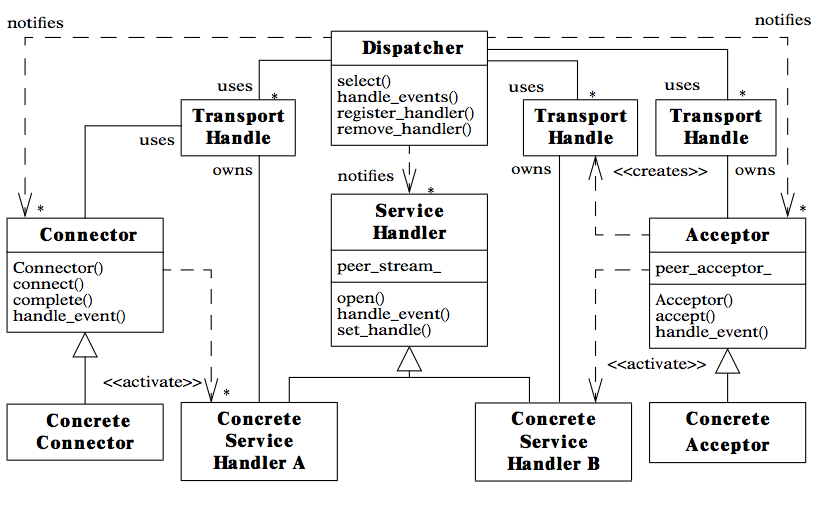
\includegraphics[width=12cm]{content/posa2/acceptor-connector/images/class-diagram.png}
	\caption{Acceptor Connector Klassendiagramm}
\end{figure}


\begin{figure}[H]
	\centering
	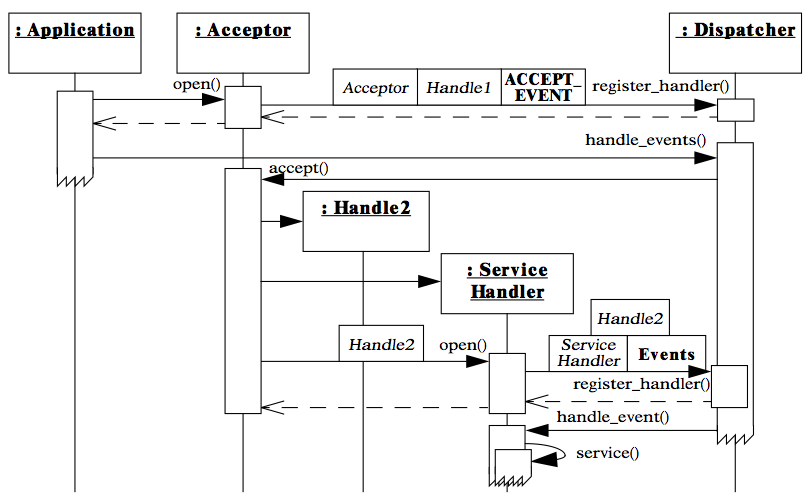
\includegraphics[width=12cm]{content/posa2/acceptor-connector/images/acceptor-ssd.png}
	\caption{Acceptor Sequenzdiagramm}
\end{figure}


\begin{figure}[H]
	\centering
	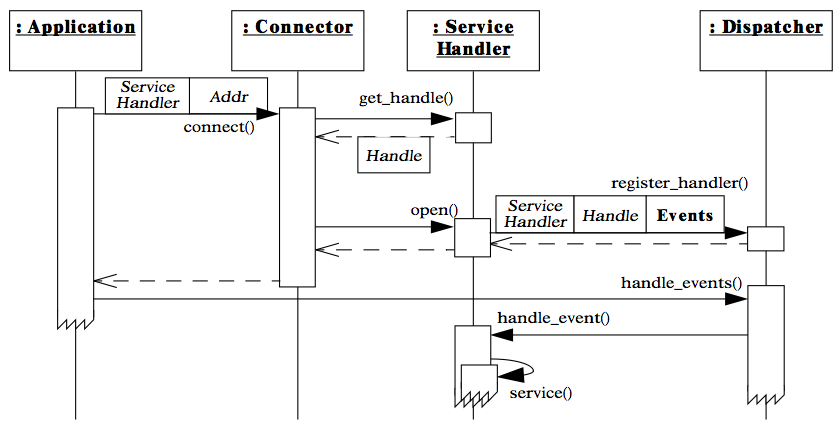
\includegraphics[width=12cm]{content/posa2/acceptor-connector/images/connector-ssd.png}
	\caption{Connector Sequenzdiagramm}
\end{figure}


\subsection{Verwendung}
\begin{itemize}
	\item Unix network superserver implementationen wie Inetd, Listen
	\item CORBA Object Request Brokers
	\item Web Browsers
\end{itemize}

\subsection{Vorteile}

Die Geringe Kopplung führt zu:
\begin{itemize}
	\item Austauschbarkeit, Wiederverwendbarkeit: Applikationscode nicht an spezifisches Transportprotokoll gebunden
	\item Portabilität: Je nach Plattform kann anderer Acceptor- und Connector-Code verwendet werden; der eigentlich Applikationscode muss nicht angepasst werden
	\item Robustheit: Kein low-level Gebastel im Applikationscode
\end{itemize}


\subsection{Nachteile}
\begin{itemize}
	\item Indirection: evt. Overhead
	\item Komplexität: für simple Applikationen ist das Pattern unter Umständen ungeeignet
\end{itemize}

\subsection{Examples}

Ein Telefongespräch zwischen zwei Managern wird durch ihre jeweiligen Büroangestellten initialisiert (Acceptor / Connector). Sobald die Verbindung steht, können die Manager (Service Handlers) miteinander sprechen.

\subsection{Prüfungsfragen}
\begin{itemize}
	\item Was ist der Unterschied zwischen Acceptor und Connector?
	\begin{itemize}
		\item ...
	\end{itemize}
\end{itemize}
